\documentclass[12 pt]{article}

%---------------- Letter Paper --------------------%
% be sure to change in document class too
\textwidth = 6.5 in
\textheight = 9.0 in
\oddsidemargin = 0.0 in
\evensidemargin = 0.0 in
\topmargin = -0.1 in
%\bottommargin = -0.5 in
\headheight = 0.0 in
\headsep = 0.2in
\parskip = 0.2in
\parindent = 0.0in

% The following packages can be found on http:\\www.ctan.org
\usepackage{graphics}
\usepackage{graphicx}
\usepackage{epsfig}
\usepackage{mathptmx}
\usepackage{times}
\usepackage{amsmath}
\usepackage{amssymb}
\usepackage{siunitx}
\usepackage{multirow}
\usepackage{booktabs}
\usepackage{longtable}
\usepackage{rotating}
\usepackage{textcomp}
\usepackage{bm}
\usepackage{fancyhdr}
\usepackage{comment}
\usepackage{subcaption}
\usepackage[linecolor=black,backgroundcolor=lightgray]{todonotes}
\usepackage[colorlinks=true, linkcolor=black, citecolor=black, urlcolor=blue]{hyperref}
\usepackage{enumitem}

\begin{document}
\begin{center}
{\LARGE \bf Autonomous Vehicles for Coastal Preservation}

% author names and affiliations
\textbf{Team Type: University Team}\\
\textbf{Team Name: Ragin' Cajuns}\\
\textbf{Region: North America}\\
\textbf{Category: Robotics}\\
\textbf{Team Members}:\\Nathan Madsen, Brennan Moeller, Joseph Stevens, and Benjamin Willis\\
\vspace{0.1in}
\textbf{Faculty Advisors}:\\Yasmeen Qudsi and Joshua Vaughan \\

\vspace{0.1in}
\footnotesize{Department of Mechanical Engineering\\
University of Louisiana at Lafayette\\
Lafayette, LA USA\\
Email: joshua.vaughan@louisiana.edu}
\end{center}


\bibliographystyle{IEEEtran}
\pagestyle{plain}
%\lhead{\footnotesize{\textit{Ragin' Cajun RoboBoat}}}
%\rhead{\footnotesize{}}
\cfoot{\thepage}

%%%%%%%%%%%%%%%%%%%%%%%%%%%%%%%%%%%%%%%%%%%%%%%%%%%%%%%%%%%%%%%%%%%%%%%%
%%%%%%%%%%%%%%%%%%%%%%%%%%%%%%%%%%%%%%%%%%%%%%%%%%%%%%%%%%%%%%%%%%%%%%%%
\begin{abstract}
\vspace{-0.2in}
The work proposed here seeks to improve the safety and efficiency of autonomous surface vessels used to monitor wetlands through the addition of an OAK-D camera. The OAK-D would increase the efficiency of the autonomous system by reducing the computational load on the on-board computers, thereby increasing the computational power available for both the scientific mission on the boat and the addition of more peripherals to enhance the safety.\todo{Brennan added "and the addition of more peripherals to enhance the safety" I didn't know if this is where you were going with the statement} This addition would also help improve the localization precision the surface vessel by enabling more sensors, such as LiDAR, to be added with the same computational resources and power requirements. The overall system would be able to achieve safer and more efficient coastal monitoring with the addition of an OAK-D camera. 
\end{abstract}

%%%%%%%%%%%%%%%%%%%%%%%%%%%%%%%%%%%%%%%%%%%%%%%%%%%%%%%%%%%%%%%%%%%%%%%%
%%%%%%%%%%%%%%%%%%%%%%%%%%%%%%%%%%%%%%%%%%%%%%%%%%%%%%%%%%%%%%%%%%%%%%%%
\section{Problem Statement}
\label{sec:problem_statement}
\vspace{-0.2in}
%
The Ragin' Cajuns are currently in pursuit of safer and more efficient autonomous maritime systems. More specifically, we conduct research into maritime systems like those that would be used to monitor wetlands like those commonly found in Louisiana. Such vessels reduce the burden of completing the dull and dangerous aspects of wetlands monitoring. The OAK-D camera would aid in increasing the efficiency of the proposed autonomous maritime systems by managing the bulk of the image processing. In doing so, the burden of the system's on-board processors would be reduced, allowing a larger percentage of computational resources to be dedicated to tasks such as sensor processing, data collection, navigation, and operational safety. The OAK-D camera will also help improve the machine-vision-based monitoring of the visual features that indicate coastal erosion. The improved systems can be used to increase both data fidelity and rates, thus reducing the time it takes to complete these monitoring tasks. 

%%%%%%%%%%%%%%%%%%%%%%%%%%%%%%%%%%%%%%%%%%%%%%%%%%%%%%%%%%%%%%%%%%%%%%%%
%%%%%%%%%%%%%%%%%%%%%%%%%%%%%%%%%%%%%%%%%%%%%%%%%%%%%%%%%%%%%%%%%%%%%%%%
\section{Application of the OAK-D}
\label{sec:}
\vspace{-0.2in}
%
\begin{figure}[tb]
\centering
    \begin{subfigure}{0.48\columnwidth}
    \centering
    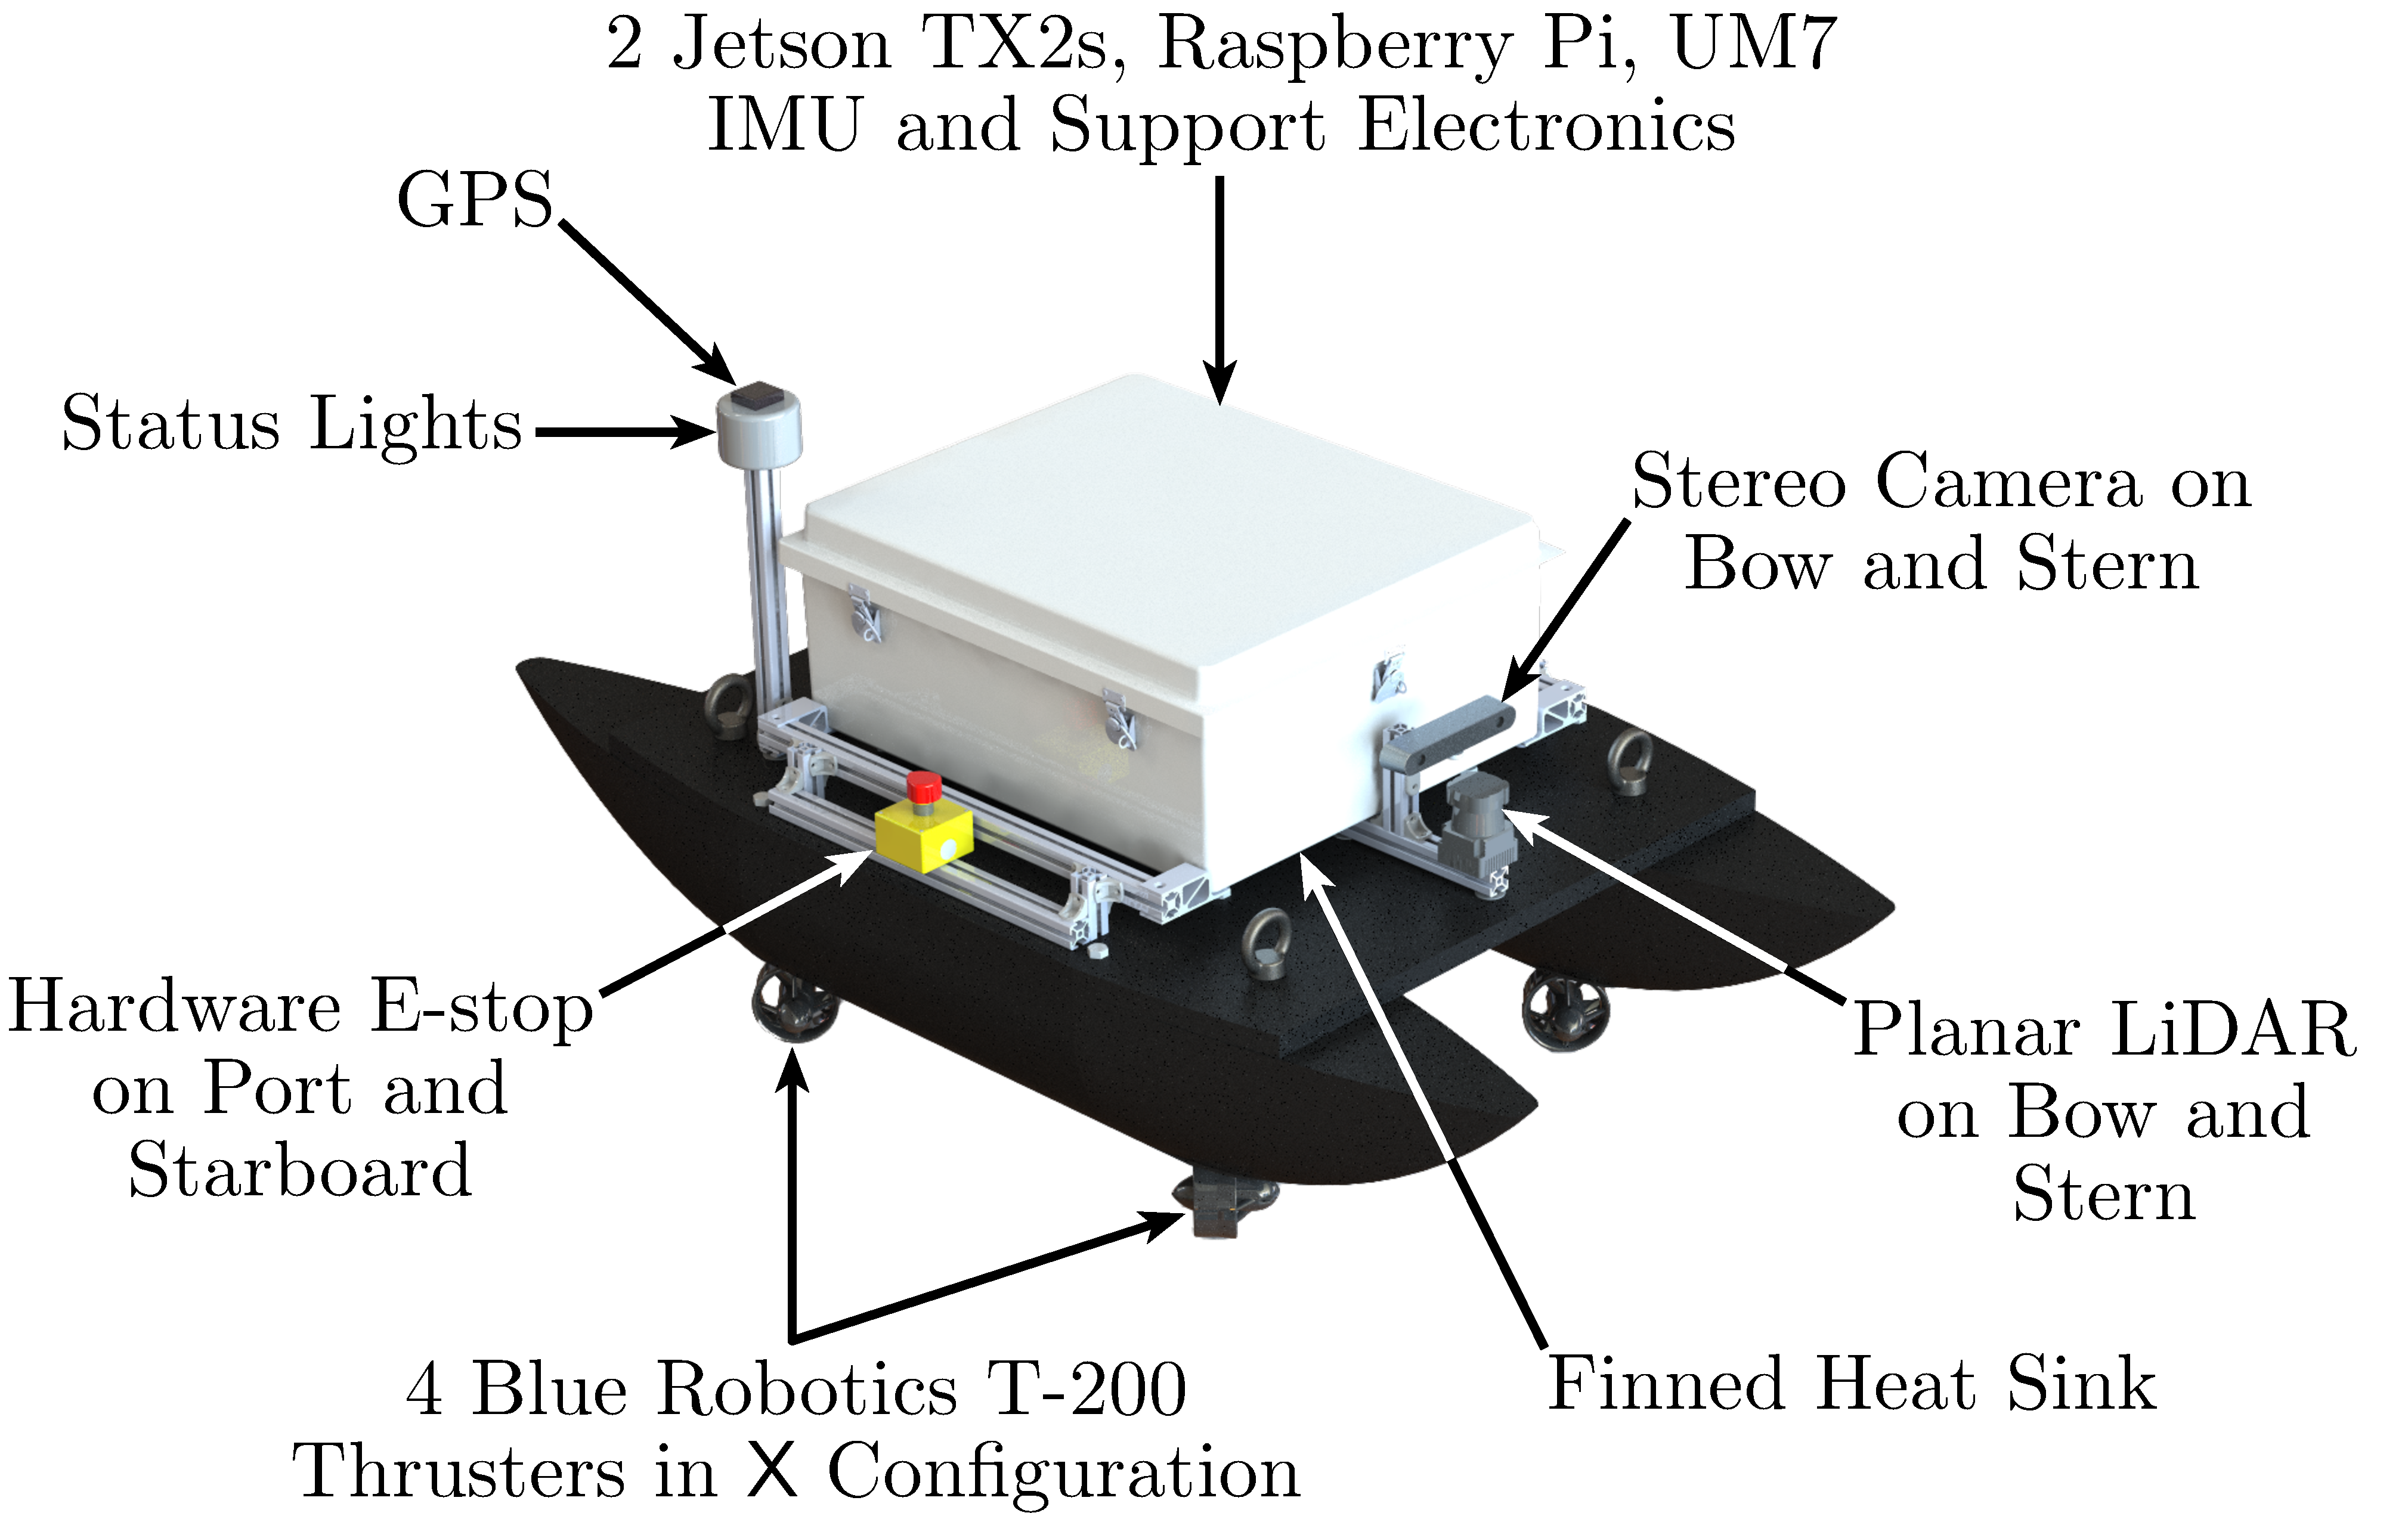
\includegraphics[width=\columnwidth]{figures/Catamaran_Final_Render_3.pdf}
	\caption{CAD Model}
    \label{fig:roboboat_CAD}
    % \vspace{0.1in}  % Optionally add some vertical spacing between subfigures
    \end{subfigure}
%
\hspace{0.02\columnwidth} % Optionally add some space between side-by-side figs
%
    \begin{subfigure}{0.48\columnwidth}
    \centering
    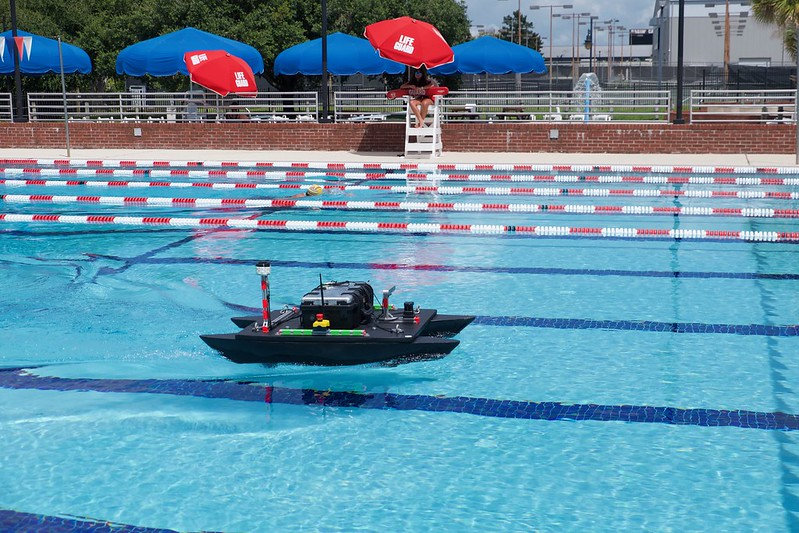
\includegraphics[width=\columnwidth]{figures/PoolTesting.jpg}  
    \caption{Testing in the UL Lafayette Pool}
    \label{fig:RoboBoat_pool}
    % \vspace{0.1in}  % Optionally add some vertical spacing between subfigures  
    \end{subfigure}
\caption{UL Lafayette Ragin' Cajuns RoboBoat} % Full figure caption
\label{fig:RoboBoat}	% Full figure label
%\vspace{-0.2in}
\end{figure}
%
One system the Ragin' Cajuns are using as a platform for research into this problem is the autonomous surface vessel (ASV) shown in Figure \ref{fig:RoboBoat}. This vessel was initially designed and built at the University of Louisiana at Lafayette for entry into the 2019 RoboNation RoboBoat competition. At the competition, it won the \href{https://mechanical.louisiana.edu/news-events/news/20190627/university-team-earns-manufacturing-award-international-roboboat}{manufacturing award} for the hull's design. 

In 2020, RoboNation held a virtual competition where the \href{https://crawlab.github.io/RoboBoat-2020/} {Ragin' Cajuns} placed 2nd overall. The team was graciously featured on \href{https://clearpathrobotics.com/blog/2020/11/research-team-uses-clearpath-simulation-in-second-place-finish-at-roboboat-2020/}{Clearpath Robotics' website} where the advancements that were made to the system by leveraging their systems for testing were publicized. 

The boat's object detection algorithms have been in constant development since its initial construction. In this system, in addition to being used for obstacle detection and object identification, the OAK-D camera would be used to aid in the simultaneous localization and mapping (SLAM) of the vessel. The OAK-D's data would be used in conjunction with RTK-GPS and LiDAR data to improve the localization precision. 

Another application of the OAK-D camera within the proposed system is on an unmanned aerial vehicle (UAV) that is currently being developed to integrate with maritime system. This camera would allow for the UAV to improve its autonomous flight by reducing the processing burden of the on-board computer. This would enable more processing time to be spent on increasing the UAV's ability to be robust to varying operating conditions rather than processing images, tracking objects, and classifying images. Due to weight constraints, most of the processing for the current visual peripherals must be carried out on the autonomous surface vessel. The OAK-D would allow for the recognition and tracking of the buoys to be done on-board the UAV. This has the benefits of both reducing the lag time for processing and reducing the required network bandwidth. The reduced lag time in vision processing will improve the safety of the UAV, while the newly-freed bandwidth can be dedicated to scientifically-relevant data.

To demonstrate the proposed system and algorithms, the OAK-D camera will be used in the 2021 RoboBoat contest. Use in the RoboBoat competition will enable testing and verification of the proposed algorithms in unknown, dynamic environments. The addition of the camera would give Ragin' Cajuns the ability to improve the autonomous system for the RoboBoat competition, and more importantly, it would enable the Ragin' Cajuns to work towards safer coastal preservation for wetlands like those found in Louisiana.

%%%%%%%%%%%%%%%%%%%%%%%%%%%%%%%%%%%%%%%%%%%%%%%%%%%%%%%%%%%%%%%%%%%%%%%%
%%%%%%%%%%%%%%%%%%%%%%%%%%%%%%%%%%%%%%%%%%%%%%%%%%%%%%%%%%%%%%%%%%%%%%%%
\section{Team Capabilities and Prior Work}
\label{sec:capability}
\vspace{-0.2in}
%
The members of this team are part of the \href{https://userweb.ucs.louisiana.edu/~jev9637/}{CRAWLAB} at the University of Louisiana at Lafayette. Research in the CRAWLAB ranges from vibration control of cranes and cable driven systems to industrial automation to mobile robotics. The foundation of this work is in conventional controls theory. However, recent work includes leveraging this conventional controls expertise with modern machine-learning-based methods. The overall aim is to reduce training times while improving the interpretability of the resulting models. These methods have been applied to both vibration control and gait design for walking robots.

Within the lab, machine-learning-based methods have been extensively used for perception and localization. For example, pipelines have been developed to identify buoys and other objects found in the \href{https://roboboat.org}{RoboBoat} and \href{https://robotx.org}{RobotX} contests, using ensembles of object detection models. For example, Figure \ref{fig:RobotX_example} shows the results from an object detection model trained to recognize the competition components in the Maritime RobotX challenge. A variant of this model was used in Figure \ref{fig:RoboBoat_example} to identify the locations of (round) buoys, whose bounding boxes are marked in white in the figure. This identification pipeline is in the process of being merged with other sensor data to improve the localization performance of the autonomous maritime systems on which it is deployed.
%
\begin{figure}[tb]
\centering
    \begin{subfigure}{0.48\columnwidth}
    \centering
    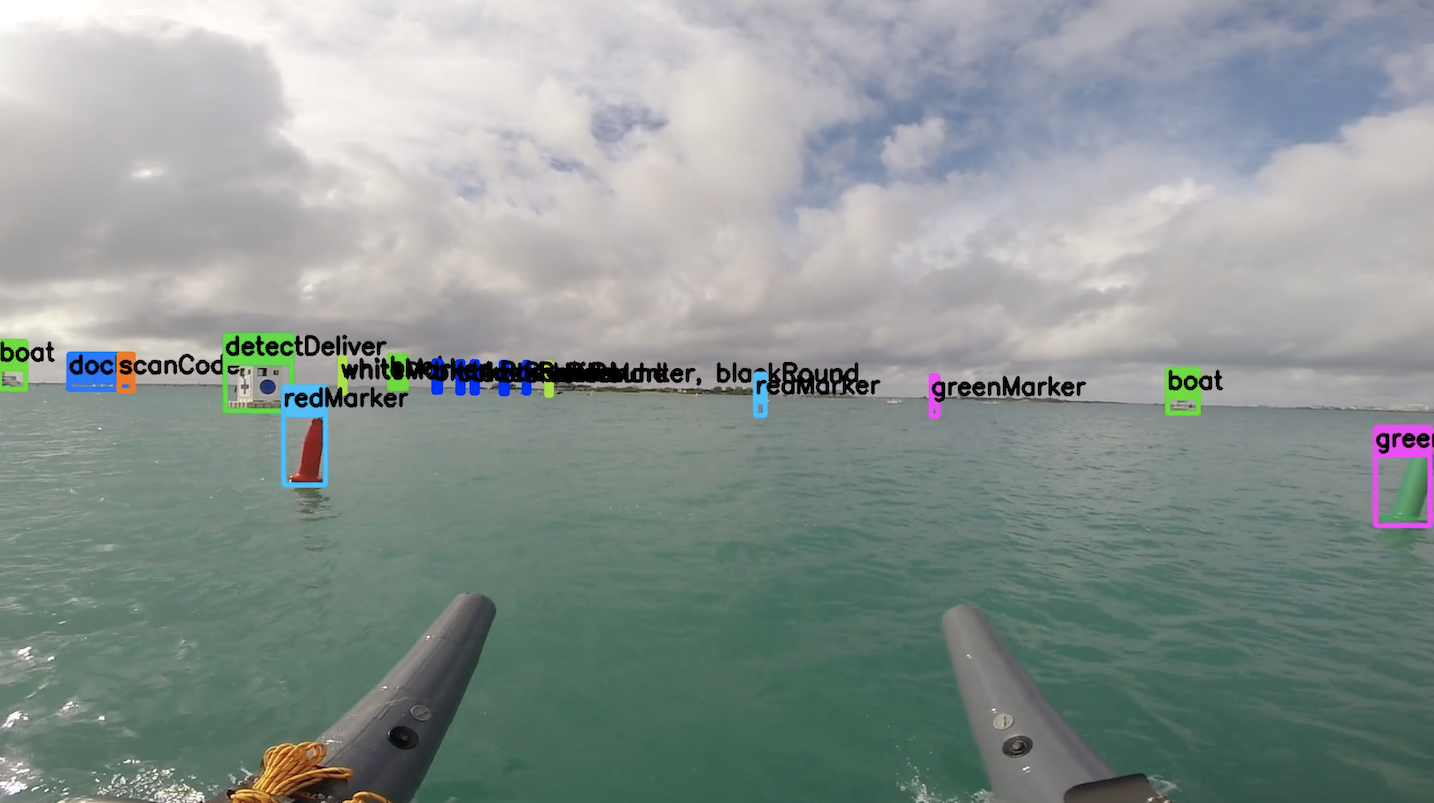
\includegraphics[width=\columnwidth]{figures/RobotX_YOLO_example.png}  
    \caption{At the Maritime RobotX Challenge}
    \label{fig:RobotX_example}
    % \vspace{0.1in}  % Optionally add some vertical spacing between subfigures
    \end{subfigure}
%
\hspace{0.02\columnwidth} % Optionally add some space between side-by-side figs
%
    \begin{subfigure}{0.48\columnwidth}
    \centering
    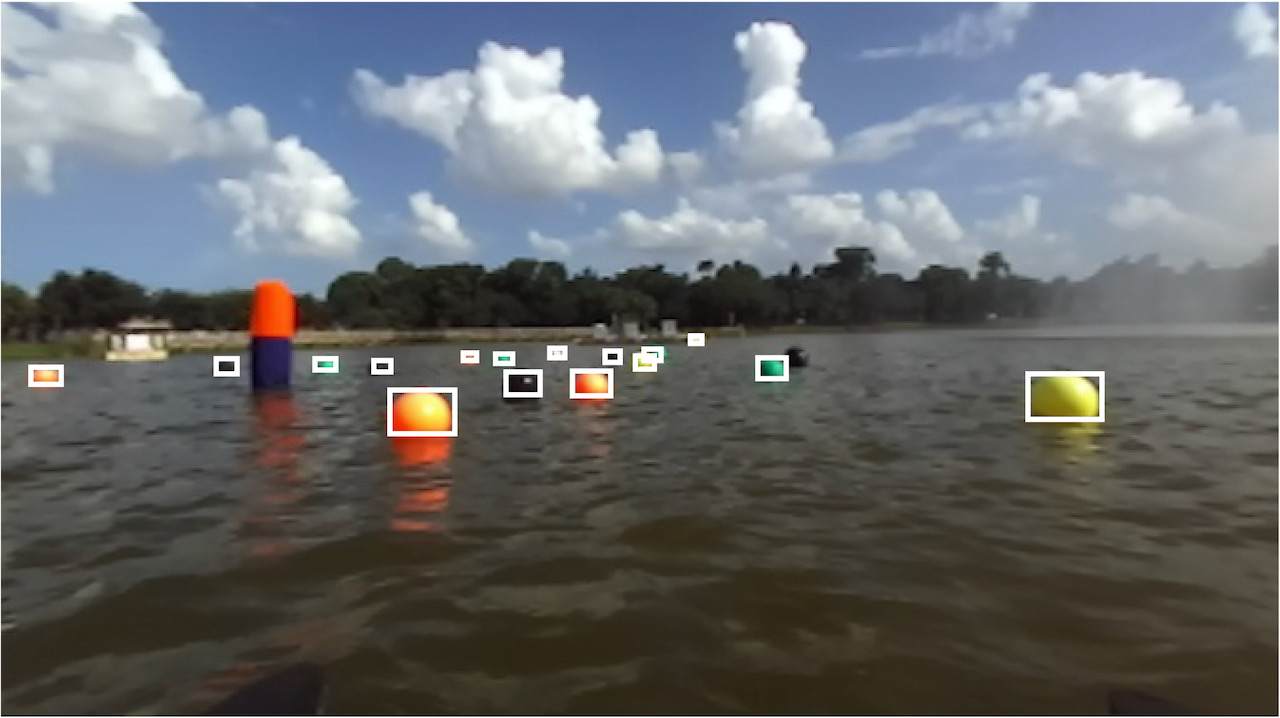
\includegraphics[width=\columnwidth]{figures/RoboBoat2019_YOLO_obstacle.jpeg}  
    \caption{At the RoboBoat Contest}
    \label{fig:RoboBoat_example}
    % \vspace{0.1in}  % Optionally add some vertical spacing between subfigures  
    \end{subfigure}
\caption{Example Performance of the UL Lafayette Object Detection Algorithms} % Full figure caption
\label{fig:detection_examples}	% Full figure label
%\vspace{-0.2in}
\end{figure}
%

In addition, there are many systems and hardware within the CRAWLAB to support the development and implementation of safe and efficient autonomous systems. There are two autonomous surface vessels (ASVs), a sixteen-foot WAM-V from Marine Advanced Research and the custom, smaller ASV discussed above. Work is currently underway to integrate an unmanned aerial vehicle (UAV) with the smaller ASV. In addition, there is a GPU server with four TITAN XP GPUs to aid in training and evaluating the models developed through this project.


%%%%%%%%%%%%%%%%%%%%%%%%%%%%%%%%%%%%%%%%%%%%%%%%%%%%%%%%%%%%%%%%%%%%%%%%
%%%%%%%%%%%%%%%%%%%%%%%%%%%%%%%%%%%%%%%%%%%%%%%%%%%%%%%%%%%%%%%%%%%%%%%%
\section{Proposed Timeline}
\label{sec:timeline}
\vspace{-0.2in}
%
To ensure the success of this proposal, a working time line has been created to ensure each aspect of the project gets completed in a timely manner. To train a real-time Convolutional Neural Network (CNN), an extensive data set of the objects that will be encountered in the competition will be created in Blender, a 3D computer graphics software, by mid-March. This will allow the Ragin' Cajuns to spend the rest of March and beginning of April properly labeling and training the CNN. Subsequently, the rest of April and beginning of May would be spent enhancing the SLAM algorithms needed on both the ASV and UAV. Following the completion of this, the installation and setup of the OAK-D camera will take place. This would be completed by mid-May. Testing of the autonomous system at RoboBoat 2021 would be completed mid-June. Finally, evaluations and documentation of the performance of the system would be completed by the end of June. 

%%%%%%%%%%%%%%%%%%%%%%%%%%%%%%%%%%%%%%%%%%%%%%%%%%%%%%%%%%%%%%%%%%%%%%%%
%%%%%%%%%%%%%%%%%%%%%%%%%%%%%%%%%%%%%%%%%%%%%%%%%%%%%%%%%%%%%%%%%%%%%%%%
\section{Additional Information}
\label{sec:additional}
\vspace{-0.2in}
%
Below are links to more information, images, and videos that demonstrate the past work of this team and its capabilities. 

\textbf{flickr Albums}
\vspace{-0.2in}
\begin{itemize}[noitemsep,nolistsep]
	\item 2016 Maritime RobotX -- \url{https://flic.kr/s/aHskDeg5Um}
	\item 2018 Maritime RobotX -- \url{https://flic.kr/s/aHskyLDzbP} \\(\textit{Note:} Team members attended, but we were unable to compete due to lack of funding.)
	\item 2019 RoboBoat -- \url{https://flic.kr/s/aHsmBqcr84}
	\item 2020 RoboBoat -- \url{https://flic.kr/s/aHsmFtTbBs}
	\item 2021 RoboBoat -- \url{https://flic.kr/s/aHsmQ9ZEPo}
	\item Other lab research -- \url{https://www.flickr.com/photos/crawlab/albums}
\end{itemize}

\textbf{Video}
\vspace{-0.2in}
\begin{itemize}[noitemsep,nolistsep]
	\item RoboBoat Autonomous Navigation -- \url{https://vimeo.com/393330950}
	\item RoboBoat Buoy Detection -- \url{https://vimeo.com/393329770}
	\item YOLOv3 for Buoy Detection -- \url{https://vimeo.com/docvaughan/robotxyolov3}
	\item ARLISS -- \url{https://vimeo.com/channels/ularliss}
\end{itemize}
	
\textbf{Other Links}
\vspace{-0.2in}
\begin{itemize}[noitemsep,nolistsep]
	\item Lab webpage -- \url{https://userweb.ucs.louisiana.edu/~jev9637/}
	\item Lab GitHub -- \url{https://github.com/crawlab}
\end{itemize}
\end{document}
